\documentclass{article}

\usepackage[utf8]{inputenc}
\usepackage{amsmath}
\usepackage[finnish]{babel}
\usepackage{hyperref}
\usepackage{graphicx}
\usepackage{listings}
\usepackage{color}

\setlength{\parindent}{0.0in}
\setlength{\parskip}{0.1in}

\definecolor{dkgreen}{rgb}{0,0.6,0}
\definecolor{gray}{rgb}{0.5,0.5,0.5}
\definecolor{mauve}{rgb}{0.58,0,0.82}

\lstset{ %
  backgroundcolor=\color{white},  % choose the background color; you must add \usepackage{color} or \usepackage{xcolor}
  basicstyle=\ttfamily\scriptsize,       % the size of the fonts that are used for the code
  breaklines=true,                % sets automatic line breaking
  commentstyle=\color{dkgreen},   % comment style
  deletekeywords={...},           % if you want to delete keywords from the given language
  escapeinside={\%*}{*)},         % if you want to add LaTeX within your code
  %frame=single,                   % adds a frame around the code
  keywordstyle=\color{blue},      % keyword style
  numberstyle=\tiny\color{gray},  % the style that is used for the line-numbers
  rulecolor=\color{black},        % if not set, the frame-color may be changed on line-breaks within not-black text (e.g. comments (green here))
  stringstyle=\color{mauve},      % string literal style
  showspaces=false,
  showstringspaces=false,
  literate={ö}{{\"o}}1
           {ä}{{\"a}}1,
  language=SQL,
  morekeywords={SERIAL}
}

\title{Tietokantojen perusteet 2013, Pershowspaces=false,   iodi III \\ Kirjastotietokanta}
\author{Mika Viinamäki \\ Paavo Rohamo \\ John Lång \\ Eero Antila \\ Juha Koiranen}

\begin{document}
\maketitle 

\section{Tietosisältökartoitus}

Tietokohteet \textbf{lihavoituna}, attribuutit \textit{kursivoituna}.

Kirjaston kokoelmissa on noin 120000 eri \textbf{kohdetta}. Suurin osa kohteista on \textit{lainattavia}, mutta osa kuuluu käsikirjastoon. Erilaisia \textbf{nimikkeitä} on noin 80000. Kullakin nimikkeellä on \textit{tunnus}, \textit{nimi} ja \textit{tyyppi}. Lisäksi nimikkeeseen voi liittyä runsaasti erilaista \textbf{kuvailutietoa}, esimerkiksi tekijä, kustantaja, sivulukumäärä, jne. Kullakin \textbf{kuvailutietotyypillä} on yksikäsitteinen tunnus. Esimerkiksi kustantajatiedon \textit{tyyppitunnus} on PUBL. \textbf{Nimiketyyppi}kohtaisesti (tyyppejä esimerkiksi kirja ja elokuva) on määritelty, mitä kuvailutietoja kyseisen tyypin nimikkeisiin liittyy sekä mitkä niistä ovat \textit{pakollisia} ja mitkä valinnaisia. Uusia kuvailutietotyyppejä pitää pystyä lisäämään ja kytkemään nimikkeisiin muuttamatta tietokannan rakennetta. Kuvailutietoja käytetään lähinnä nimiketietojen haussa.

Kohdekohtaiset tiedot eivät riipu kohteen tyypistä. Kullakin kohteella on yksikäsitteinen \textit{tunnusnumero}. Lisäksi kohteesta säilytetään \textbf{sijaintitietoa} (\textit{osasto}, \textit{hyllykkö}, \textit{hylly}) ja tietoa \textit{hankinta-ajankohdasta} ja \textit{hankintahinnasta}.

Kirjaston asiakaskunta muodostuu noin 20000 \textbf{asiakkaasta}. Asiakkaasta on taltioitu \emph{normaalit asiakastiedot}. Asiakkaalla on yksikäsitteinen \emph{asiakasnumero}. Asiakkaat voivat \textbf{lainata} kohteita. He voivat myös \textbf{tilata} nimikkeitä. Palautuksen yhteydessä järjestelmä ilmoittaa ensimmäiselle jonottavalle asiakkaalle kohteen saapuomisesta. Lainasta tallennetaan \emph{lainausajankohta} ja \emph{palautuspäivä}. Lainaustietoihin voi liittyä myös \emph{karhuamismerkintöjä}. Kun laina palautetaan, lainaustietoa ei poisteta, vaan se jää kantaan historiatiedoksi. 

\section{Käsitekaavio}

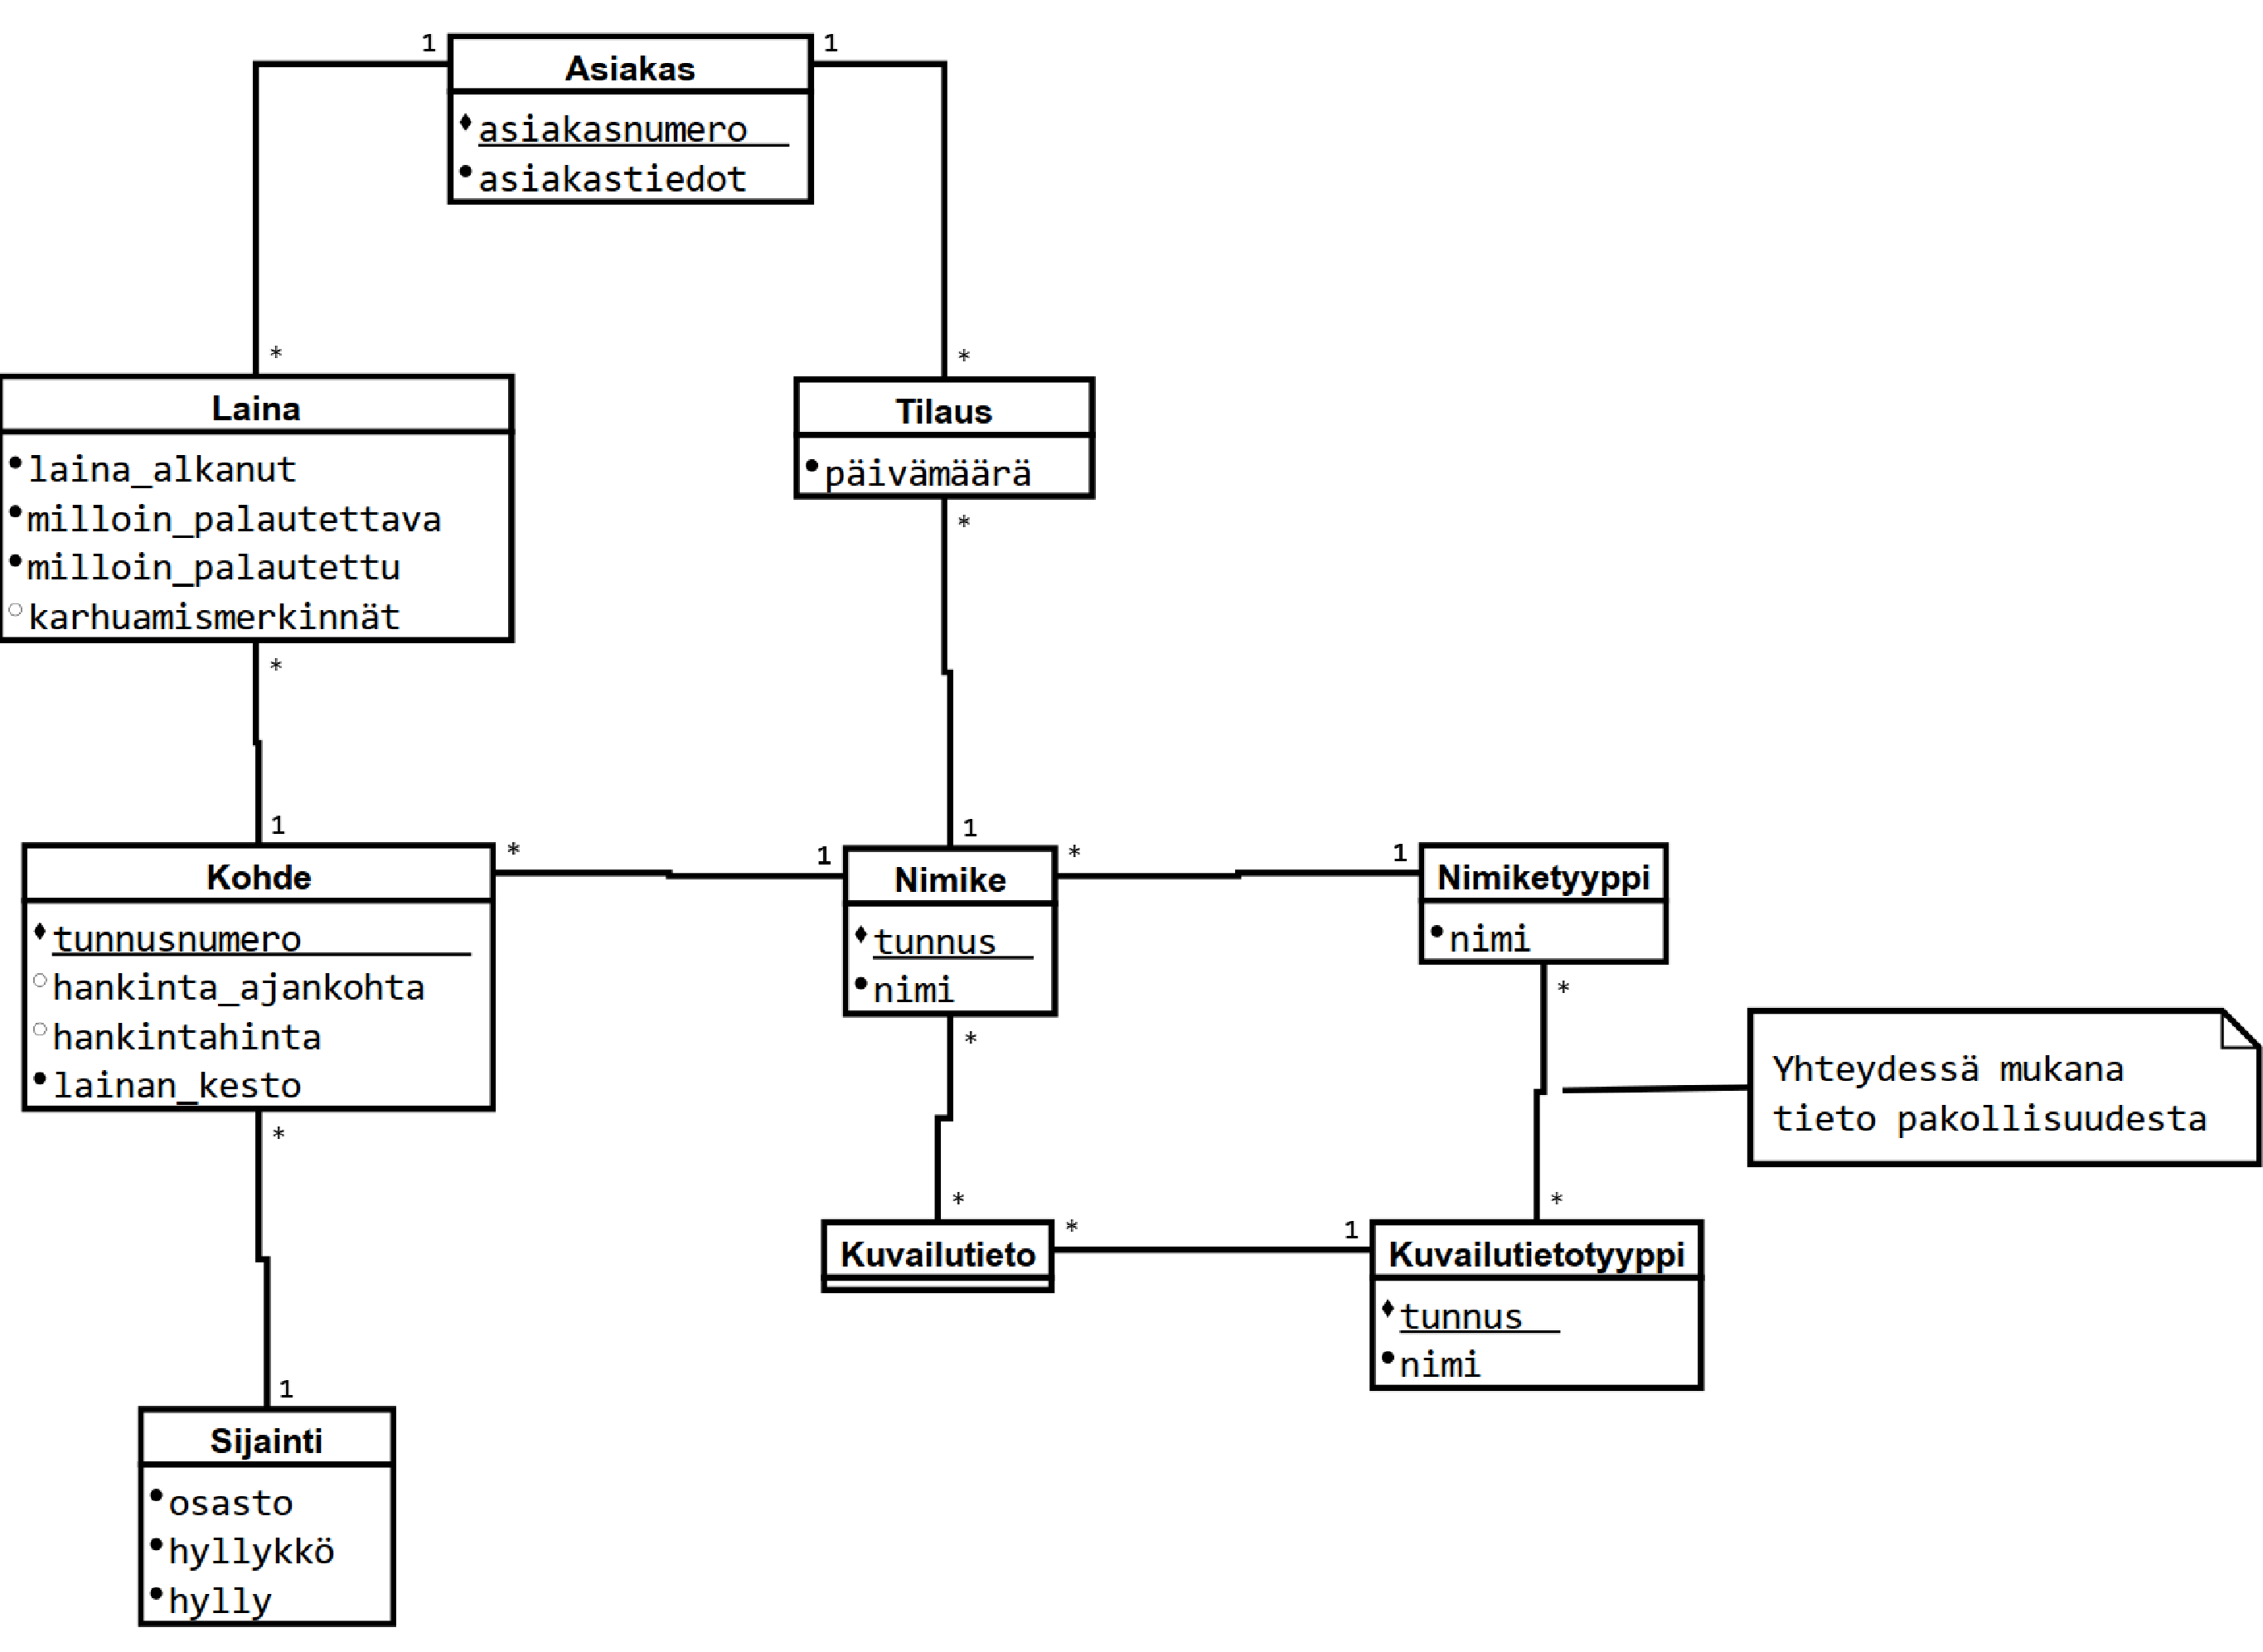
\includegraphics[width=\linewidth]{../kaaviot/kasitekaavio.pdf}

Nimike kuvaa jotain kirjaston valikoimissa olevaa teosta, ja kohde kuvaa yhtä fyysistä kopiota jostain tällaisesta nimikkeestä.

Nimiketyyppi kuvaa jotain muotoa, jota nimike edustaa - esimerkiksi kirja tai elokuva. Jokaiseen nimiketyyppiin liittyy tietyt kuvailutietotyypit, jotka voivat olla pakollisia tai vapaaehtoisia. Kuvailutieto tarkoittaa jotain nimikkeeseen liittyvää tietoa, kuten esimerkiksi nimikkeen kustantajaa tai ohjaajaa. Kuvailutietotyyppi kuvaa tämän tiedon tyyppiä.

Tilaus kuvaa varausta johonkin nimikkeeseen.

\section{Tietokantakuvaus}

\subsection{Tietokantakaavio}

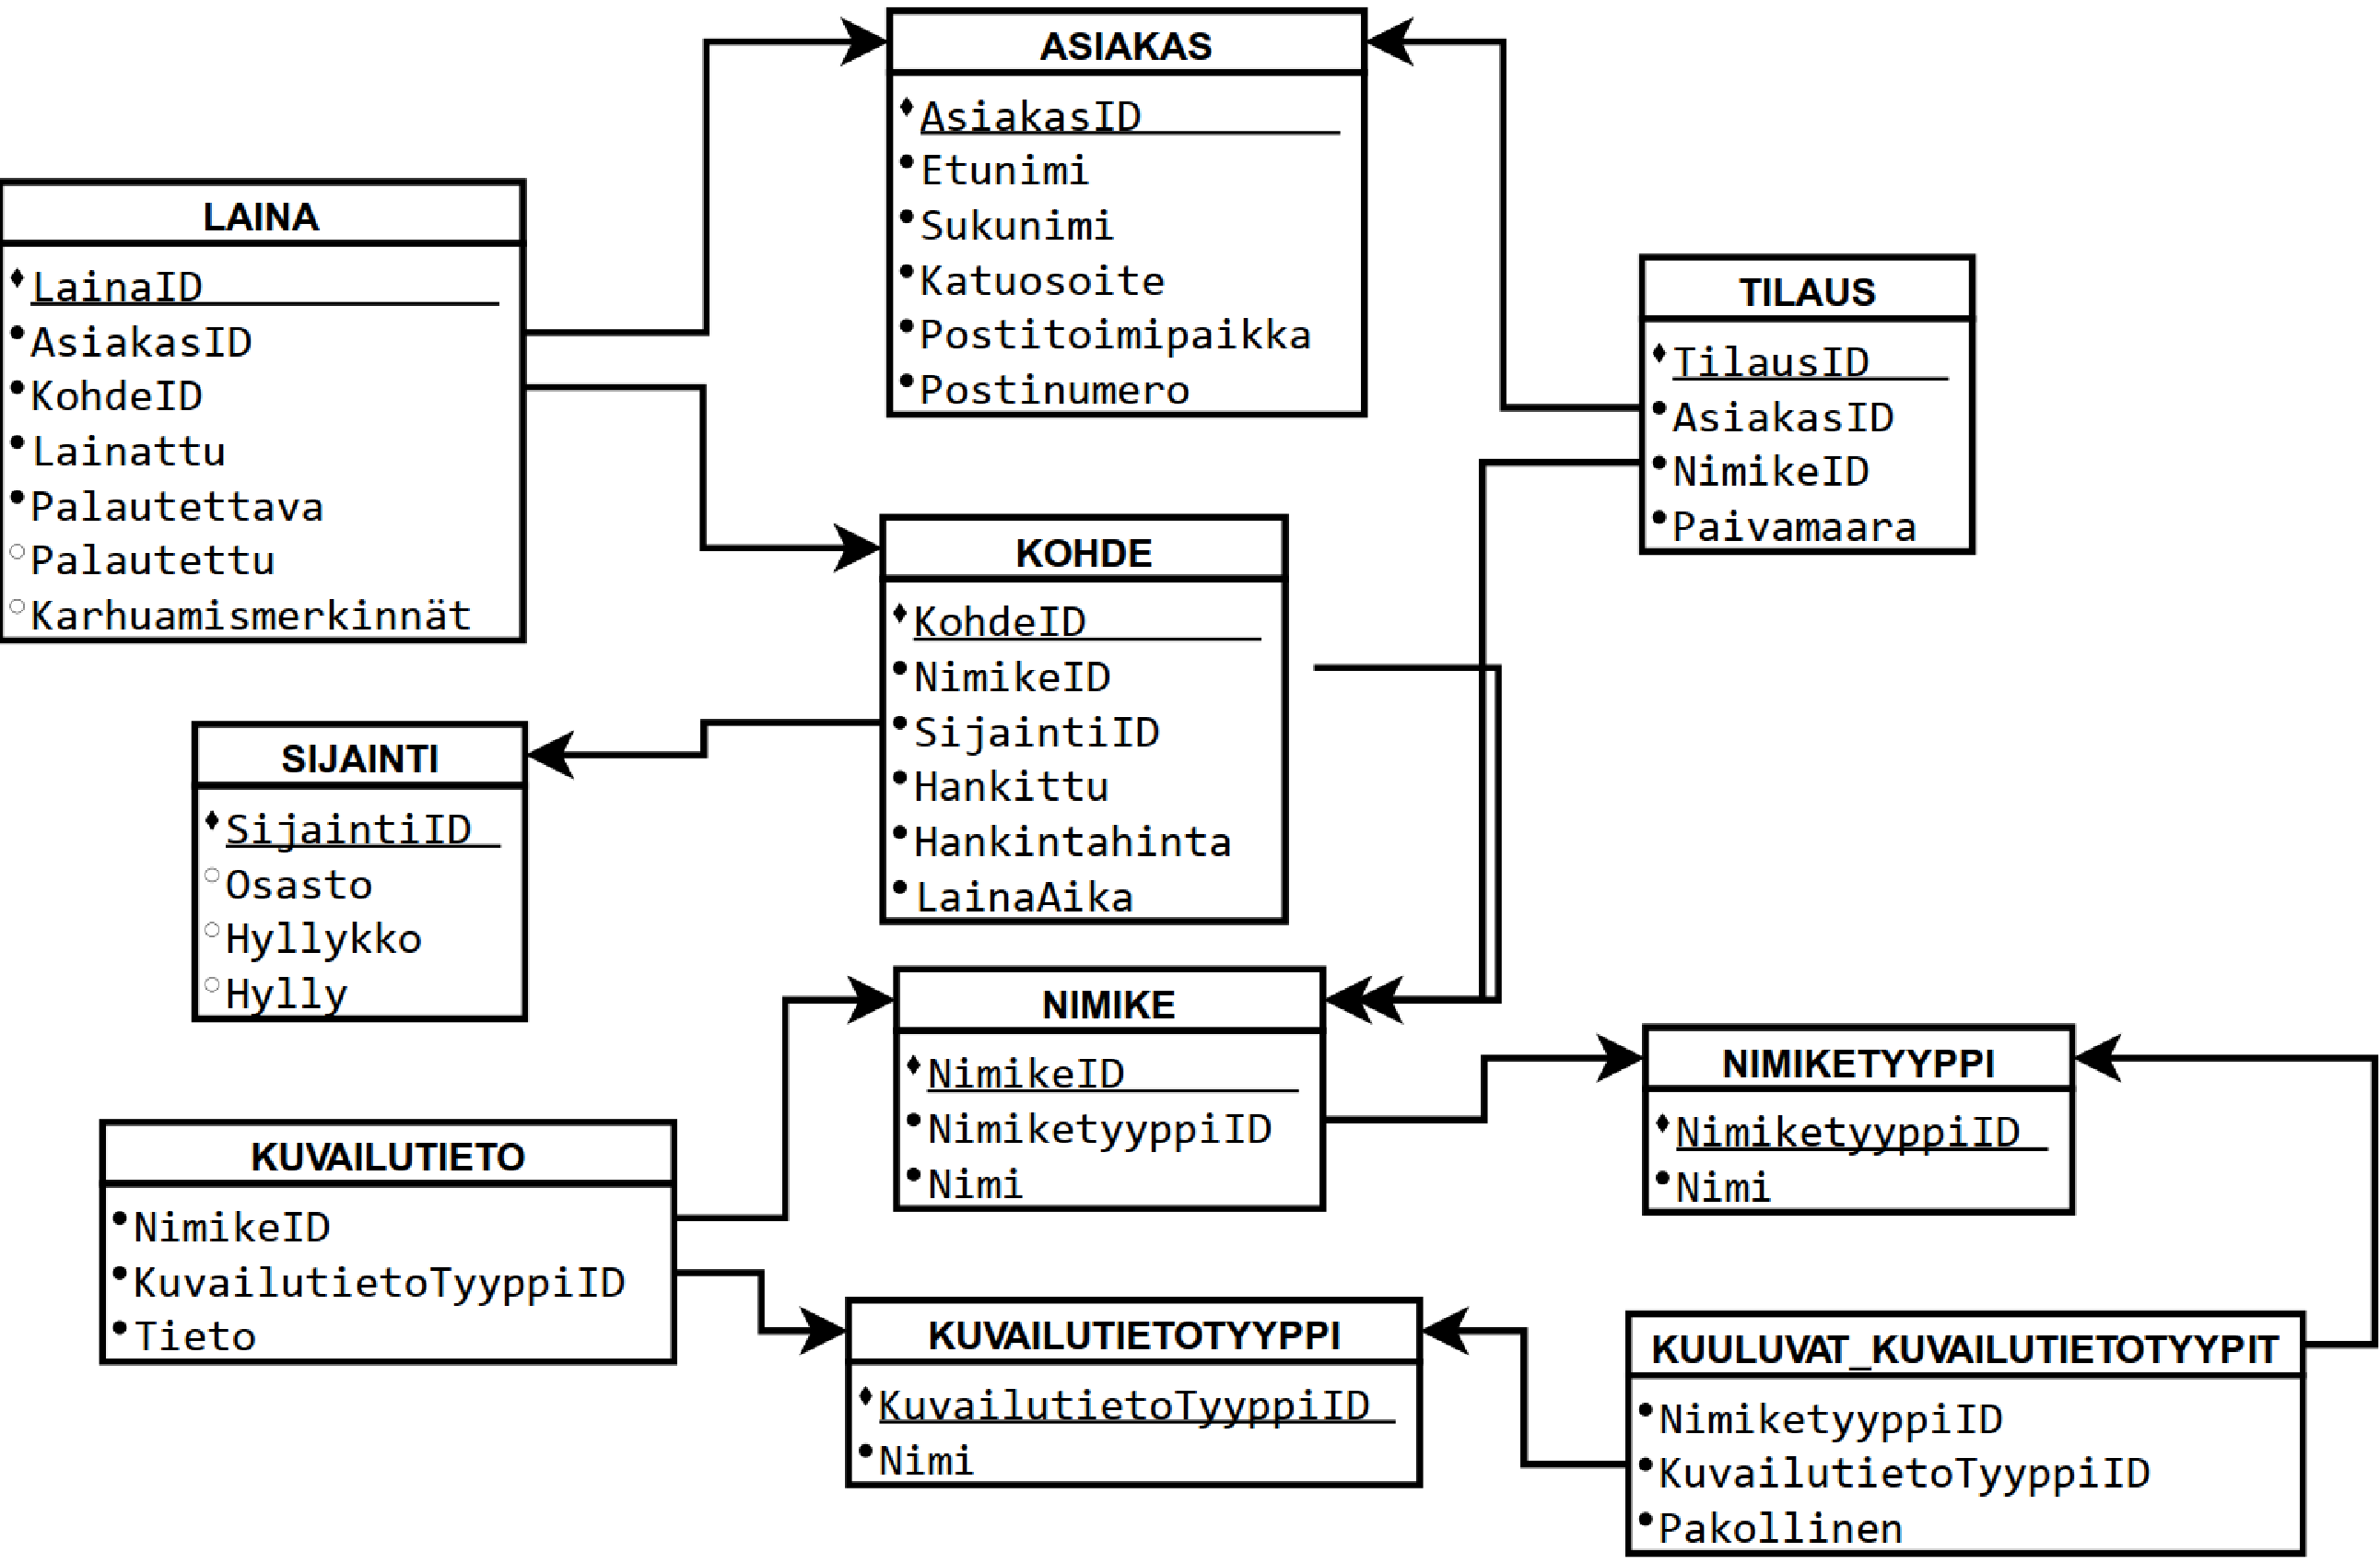
\includegraphics[width=\linewidth]{../kaaviot/tietokantakaavio.pdf}

\subsection{SQL-lauseet}

Kaikki tämän dokumentin SQL-lauseet olettavat käytössä olevan PostgreSQL-tietokantaohjelmiston tuoreehko versio (testattu versiolla 9.2.3).

\lstinputlisting{../sql/create_tables.sql}

\section{Riippuvuusanalyysi}

\textbf{Asiakas:} Taulussa on funktionaalisia riippuvuuksia esimerkiksi postinumerolla ja postitoimipaikalla - jälkimmäinen riippuu suoraan ensimmäisestä. Taulu ei siis täytä kolmatta normaalimuotoa.

\textbf{Sijainti, Nimiketyyppi, Nimike, Kuvailutietotyyppi, Kuuluvat\_\-Kuvailutietotyypit, Kuvailutieto, Kohde, Tilaus:} Attribuuteilla ei funktionaalisia riippuvuuksia kuin pääavaimiin.

\textbf{Laina:} Palautettava-attribuutin voi päätellä lainattu-attribuutin ja Kohde-taulun laina-ajan perusteella - olettaen että kohteen laina-aika ei koskaan muutu. Kohteen laina-aika voi kuitenkin muuttua, jolloin kyseessä ei ole funktionaalinen riippuvuus.

\section{Esimerkkidata}

\lstinputlisting{../sql/initial_data.sql}

\section{Käyttötapauksia}

\subsection{Kaikkien kohteiden listaaminen}

Kaikki tietokannassa olevat kohteet, niiden nimet ja tyypit selkokielisenä sekä sijaintitiedot saa seuraavalla kyselyllä:

\begin{lstlisting}
SELECT NIMIKE.Nimi,
    NIMIKETYYPPI.Nimi,
    SIJAINTI.Osasto,
    SIJAINTI.Hyllykko,
    SIJAINTI.Hylly
FROM KOHDE
INNER JOIN NIMIKE
    ON KOHDE.NimikeID = NIMIKE.NimikeID
INNER JOIN NIMIKETYYPPI
    ON NIMIKE.NimikeTyyppiID = NIMIKETYYPPI.NimikeTyyppiID
INNER JOIN SIJAINTI
    ON KOHDE.SijaintiID = SIJAINTI.SijaintiID;
\end{lstlisting}

\end{document}